\chapter{Simuladores de tráfico y sistemas multiagente}
\label{ch:sota-traffic-simulators-and-mas}

Se pretende desarrollar un método para el análisis de la eficiencia de los conductores, realizando para ello un modelo del perfil de conducción a partir de técnicas de Inteligencia Computacional y aplicándolo en un entorno multiagente de donde obtener el resto de parámetros. Así, una vez configurado el entorno multiagente, se podrá simular el tráfico y el comportamiento de los conductores dentro de éste cuando su marcha está condicionada por factores como el tráfico, semáforos, etcétera.

Es para ello necesario un análisis previo del estado de la cuestión en torno a varios conceptos y su relación: la inteligencia computacional y sus técnicas, agentes y sistemas multiagente y por último, modelos de conductor y simuladores de tráfico. Esta sección se encarga de recoger el resultado de la revisión de la literatura en estos temas y sirve de base para el desarrollo de la tesis.

\section{Simulación de tráfico}

El tráfico es un sistema cuyo funcionamiento depende de multitud de factores con una organización caótica. Debido a esto, obtener modelos exactos es una tarea prácticamente imposible y es por ello que la mayoría del trabajo cuyo objetivo es la predicción se realice en base a simuladores.

Hoy en día la oferta de simuladores de tráfico existente es amplia. NO SÉ QUÉ COJONES PONER AQUÍ DE QUE SE OFERTAN CON DIFERENTES LICENCIAS, TANTO ABIERTAS COMO CERRADAS.

A lo mejor aquí hay que especificar que hablando de simuladores de tráfico, sólo vamos a centrarnos en temas de simulación de vehículos utilitarios (coches o como cojones se llamen), sin entrar en detalles de simulación de otro tipo de vehículos o de peatones.

Dentro de simulación de tráfico que no es directamente simulación de coches, se  puede hablar (para nombrar y hacer un par de párrafos con refeerncias) de la simulación para la evaluación de sistemas de señalización inteligentes\cite{jin2016evaluation}, estimación de emisiones\cite{quaassdorff2016microscale}

He encontrado un smiulador que es relativamente reciente y que puede merecer la pena mencionar (más párrafos, yuhu!). es el X10, y cero que tiene que ver con algo de IBM, y algo también de inteligencia porque hablan de preferencias para el conductor en temas deruta, evlocidad y no se qué hostias. Dejo aquí los enlaces: \url{http://x10.sourceforge.net/documentation/presentations/X10DayTokyo2015/x10daytokyo15-mizuta.pdf}, \url{http://ieeexplore.ieee.org/xpl/login.jsp?tp=\&arnumber=6365068\&url=http\%3A\%2F\%2Fieeexplore.ieee.org\%2Fxpls\%2Fabs\_all.jsp\%3Farnumber\%3D6365068}, \url{http://informs-sim.org/wsc12papers/includes/files/pos148.pdf}, \url{https://www.researchgate.net/profile/Tsuyoshi\_Ide2/publication/236173272\_X10-based\_massive\_parallel\_large-scale\_traffic\_flow\_simulation/links/00b4951b89905784a7000000.pdf}


AQUÍ ESTARÍA MUY BIEN UNA IMAGEN COMO LA QUE APARECE EN~\cite{krajzewicz2002sumo} SOBRE LOS DIFERENTES SIMULADORES.


\subsection{Microsimulación vs. macrosimulación}

Los dos puntos de vista principales a la hora de abordar un modelo de flujo de tráfico son los micromodelos y los macromodelos. Cuando se trabaja con simulaciones, dependiendo de con qué modelo se trabaje hablamos entonces de microsimulaciónes y macrosimulaciónes, o simlpemente simulaciones \textit{micro} y \textit{macro} respectivamente. Sus características son las siguientes:

\begin{itemize}
	\item \textbf{Micromodelos}. Su objetivo es estudiar desde un punto de vista de granularidad fina (e.g. vehículos o peatones) las micropropiedades del flujo de tráfico (e.g. cambio de carril, aproximaciones a vehículos delanteros o adelantamientos) para evaluar su comportamiento. Tiene dos principales ventajas, la posibilidad de estudiar el tráfico como un todo a partir de sus elementos más simlpes (ofreciendo una representacińo más fiel de este) y la posibilidad de estudiar cada elemento por separado. Sin embargo, la principal desventaja de este tipo de modelos es que cada elemento de la simulación requiere de cómputo y por tanto simulaciones con alto contenido de elementos pueden llegar a ser inviables.
	\item \textbf{Macromodelos}. Este tipo de modelos centran su esfuerzo en estudiar el flujo de tráfico como un todo, explorando sus macropropiedades (e.g. evolución del tráfico, efectos onda, velocidad media o flujo en vías). Su ventaja principal es que a nivel macroscópico permiten estudiar propiedades que a nivel microscópico requeriría una cantidad ingente de recursos. Sin embargo, es imposible obtener información precisa de un elemento en particular del tráfico.
\end{itemize}

Aunque esta es la categorización típica de modelos, en la literatura aparecen otros tipos de modelo con granularidades que pueden considerarse no pertenecientes a ninguno de estos dos conjuntos.

Por ejemplo, los \textbf{sub-micromodelos} (\TODO buscar referencia) donde la granularidad baja hasta el punto que los elementos tómicos del modelo son las propias partes del vehículo o los conductores.

Otro ejemplo son los \textbf{mesomodelos}\cite{munoz2001integrated}\cite{casas2011need} donde se trata de amortiguar los problemas interentes a la complejidad en los micromodelos y a la falta de resolución en los macromodelos (\TODO añadir una figura para el modelo citado en~\cite{munoz2001integrated}, donde se hace uso de ventanas en al vía para analizar el comportamiento micro, dejando el modelo fuera de esa ventana en la granularidad macro).

\subsection{Simulación discreta vs. continua}

La discertización aquí se refiere tanto a tiempo como a espacio.

Si hablamos de tiempo, en general las simulaciones de tiempo continuo trabajan sobre macrosimulación, por lo que es de menor interés para nosotros que los simuladores discretos de tiempo, donde se cuantifica el tiempo de la simulación, generalmente a una frecuencia de 1Hz.

Si hablamos de espacio, nos interesan más los simuladores continuos, ya que los discretos pierden demasiado detalle, y nos interesa más el comportamiento en cada instante t que la colocación relativa aproximada de los vehículos en cada instante t (cuantificado o no)

\subsection{Comparativa de simuladores}

En este apartado se facilita la comparativa realizada para la elección de simulador sobre el que basar los escenarios a plantear en las simulaciones de los modelos de conductor.

Quizá se pudea hablar del \enquote{SMARTEST} project: \url{http://www.its.leeds.ac.uk/projects/smartest/}

Simuladores de pago:

Quadstone paramics (microscopic)
VISSUM (macroscopic)
VISSIM (microscopic)
AIMSUN

Simuladores gratuitos:

Matsim
SUMO (microscopic)
Repast
MAINSIM
Synchro

Ni puta idea:

CUBE
SATURN
PARAMICS
TRANSIMS

\section{\glsentrylong{sumo}}

En definitiva, el simulador que más se adapta a nuestras necesidades y el que se usará como simulador base en el desarrollo de esta tesis será \gls{sumo}\sidenote{Sus principales publicaciones son~\cite{krajzewicz2002sumo}, \cite{behrisch2011sumo} y \cite{krajzewicz2012recent}.}. \gls{sumo} es un entorno de microsimulación de código abierto\sidenote{Licenciado bajo la \gls{gpl}, concretamente la versión $3.0$.} que implementa un modelo discreto en el tiempo y continuo en el espacio.

Además de simulación clásica, \gls{sumo} provee de una interfaz gráfica (se puede ver un pantallazo en la figura~\ref{fig:sumo-simulator}) donde se puede ver el comportamiento de cada vehículo durante la simulación. Es interesante para obtener de un vistazo información acerca del funcionamiento del modelo en concreto a controlar. Otras de las características que el simulador ofrece son las siguientes:

\begin{figure}
	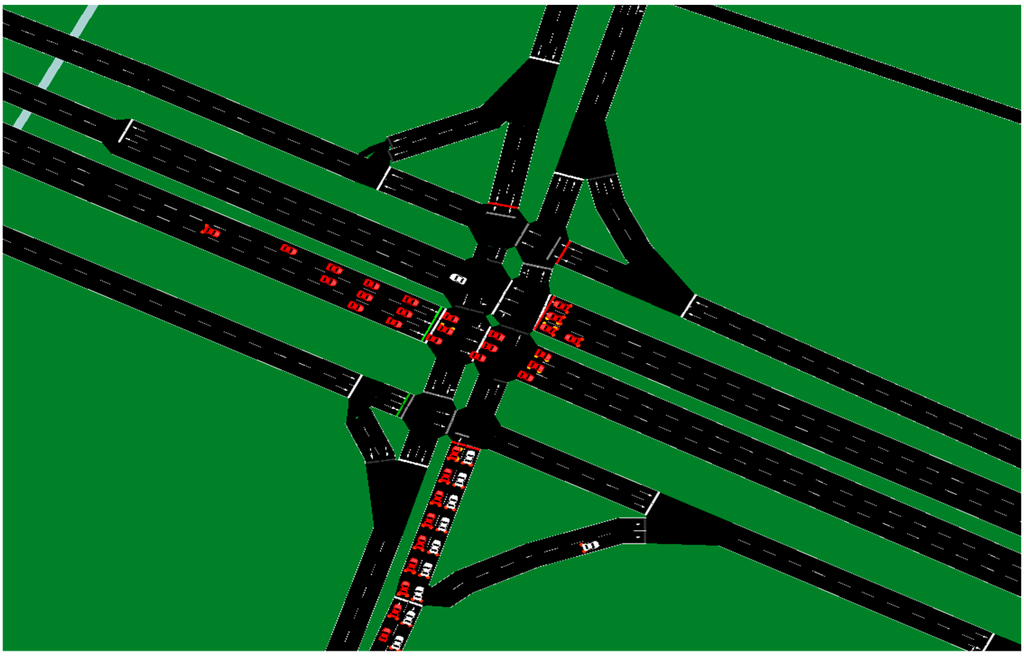
\includegraphics{sumo-simulator}
	\caption{Ejemplo de pantalla del simulador \gls{sumo}. Además de entorno de simulación propiamente dicho, \gls{sumo} provee de una interfaz gráfica que permite una visualización general, de zonas y de elementos en concreto a la vez que permite la variación de configuración de la simulación durante el desarrollo de la misma.}
	\label{fig:sumo-simulator}
\end{figure}

\begin{itemize}
	\item Multimodalidad permitiendo modelar no sólo tráfico de vehículos sino de peatones, bicicletas, trenes e incluso de barcos.
	\item Vehículos de diferentes tipologías, Simulación con y sin colisiones de vehículos.
	\item Diferentes tipos de vehículos y de carreteras, cada una con diferentes carriles y éstas con diferentes subdivisiones de subcarriles (diseño conceptual para permitir las simulaciones )
\end{itemize}

Al estar licenciado bajo la licencia \gls{gpl}, su distribución implica a su vez la distribución de su código fuente. Esto permite la modeificación de su comportamiento y el desarrollo de nuevos modelos integrados dentro del simulador. Sin embargo nosotros no haremos uso de esta característica, sino que usaremos \gls{sumo} como aplicación servidor y el módulo \gls{traci} como aplicación cliente desde donde gestionar todos los aspectos de cada simulación.

\subsection{La interfaz \glsentrylong{traci}}

\gls{traci}